%!TEX root = ../../novoIndex.tex
A tarefa de aprendizado considerada para a estimação de idade de telespectadores é a regressão. Neste contexto, uma imagem em cores RGB de dimensões $224 \times 224$ pixels contendo uma face humana centralizada será fornecida como entrada. A saída desejada é a estimativa de idade, em anos, da pessoa correspondente, conforme exemplificado na Figura \ref{fig:deniro_cnn}. Esta tarefa será abordada segundo o paradigma de aprendizado supervisionado.

\begin{figure}[!ht]
  \centering
     \caption{Tarefa de aprendizado}
     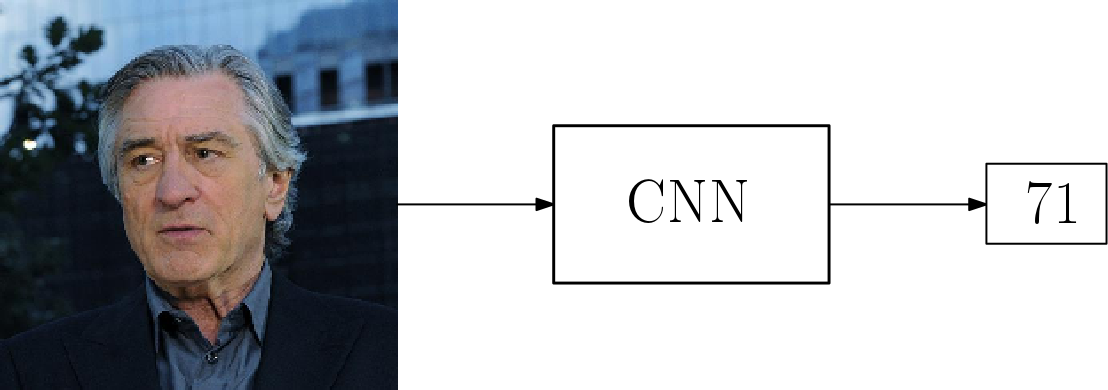
\includegraphics[width=0.8\textwidth]{img/deniro_cnn}
     \label{fig:deniro_cnn}
\end{figure}

Os dados disponíveis para este contexto serão particionados em três conjuntos disjuntos, sendo $70\%$ reservados para o treino, $10\%$ para validação e $20\%$ para teste. Esta partição obedece à tecnica \emph{Holdout} de validação cruzada \cite{brink2016real}.

%Os modelos propostos para esta tarefa terão seu desempenho aferido perante os dados do conjunto de testes de acordo com a métrica de desempenho \emph{Root Mean Squared Error} (RMSE). Esta métrica considera a diferença entre cada um dos valores previstos $\hat{y}$ e os reais $y$, e posteriormente quantifica uma média imune à variação positiva ou negativa desta diferença. A Equação \ref{eq:rmse} denota o cálculo do RMSE \cite{brink2016real}.

Os modelos propostos par aesta tarefa terão seu desempenho aferido perante os dados do conjunto de testes de acordo com duas métricas de desempenho, \emph{Root Mean Squared Error} (RMSE) e \emph{Mean Average Error} (MAE). Estas métricas são análogas na medida em que consideram a diferença entre cada um dos valores previstos $\hat{y}$ e os reais $y$, e posteriormente quantificam uma média imune à variação positiva ou negativa desta diferença. A Equação \ref{eq:rmse} denota o cálculo do RMSE, enquanto a Equação \ref{eq:mae} define o cálculo do MAE \cite{willmott2005advantages}.

\begin{equation}\label{eq:rmse}
     \textrm{RMSE} = \sqrt{\frac{1}{n} \sum_{i=1}^n (y_i - \hat{y})^2}.
\end{equation}
%\cite{willmott2005advantages}
\begin{equation}\label{eq:mae}
     \textrm{MAE} = \frac{1}{n}\sum_{i=1}^{n} |y_i - \hat{y}|
\end{equation}

O RMSE será considerado para o cálculo da perda e por conseguinte da atualização dos pesos dos modelos, enquanto o MAE será utilizado para fins de comparação do desempenho dos modelos propostos neste trabalho com os modelos consolidados na bibliografia e detalhados nos trabalhos relacionados na Seção \ref{sec:trab_relac}.
